\documentclass[a4paper,11pt,twoside]{article}
%\documentclass[a4paper,11pt,twoside,se]{article}

\usepackage{UmUStudentReport}
\usepackage{verbatim}   % Multi-line comments using \begin{comment}
\usepackage{courier}    % Nicer fonts are used. (not necessary)
\usepackage{pslatex}    % Also nicer fonts. (not necessary)
\usepackage[pdftex]{graphicx}   % allows including pdf figures
\usepackage{listings}
\usepackage{pgf-umlcd}
\usepackage{blindtext}
\usepackage{rotating}
\usepackage{enumitem}
%\usepackage{lmodern}   % Optional fonts. (not necessary)
%\usepackage{tabularx}
%\usepackage{microtype} % Provides some typographic improvements over default settings
%\usepackage{placeins}  % For aligning images with \FloatBarrier
%\usepackage{booktabs}  % For nice-looking tables
%\usepackage{titlesec}  % More granular control of sections.

% DOCUMENT INFO
% =============
\department{Department of Mathematics and Mathematical Statistics}
\coursename{Calculus in One Variable 7.5 p}
\coursecode{5MA009 HT17}
\title{Computer Laboration}
\author{Lorenz Gerber ({\tt{dv15lgr@cs.umu.se}})}
\date{2017-11-19}
%\revisiondate{2016-01-18}
\instructor{Per Åhag}


% DOCUMENT SETTINGS
% =================
\bibliographystyle{plain}
%\bibliographystyle{ieee}
\pagestyle{fancy}
\raggedbottom
\setcounter{secnumdepth}{2}
\setcounter{tocdepth}{2}
%\graphicspath{{images/}}   %Path for images

\usepackage{float}
\floatstyle{ruled}
\newfloat{listing}{thp}{lop}
\floatname{listing}{Listing}



% DEFINES
% =======
%\newcommand{\mycommand}{<latex code>}

% DOCUMENT
% ========
\begin{document}
\lstset{language=R}
\maketitle
\thispagestyle{empty}
\newpage
%\tableofcontents
%\thispagestyle{empty}
%\newpage

\clearpage
\pagenumbering{arabic}

\section{Plot of the function $f(x) = x^{11}-5x^2+e^x-5$}

\begin{figure}[h!]
  \centering
  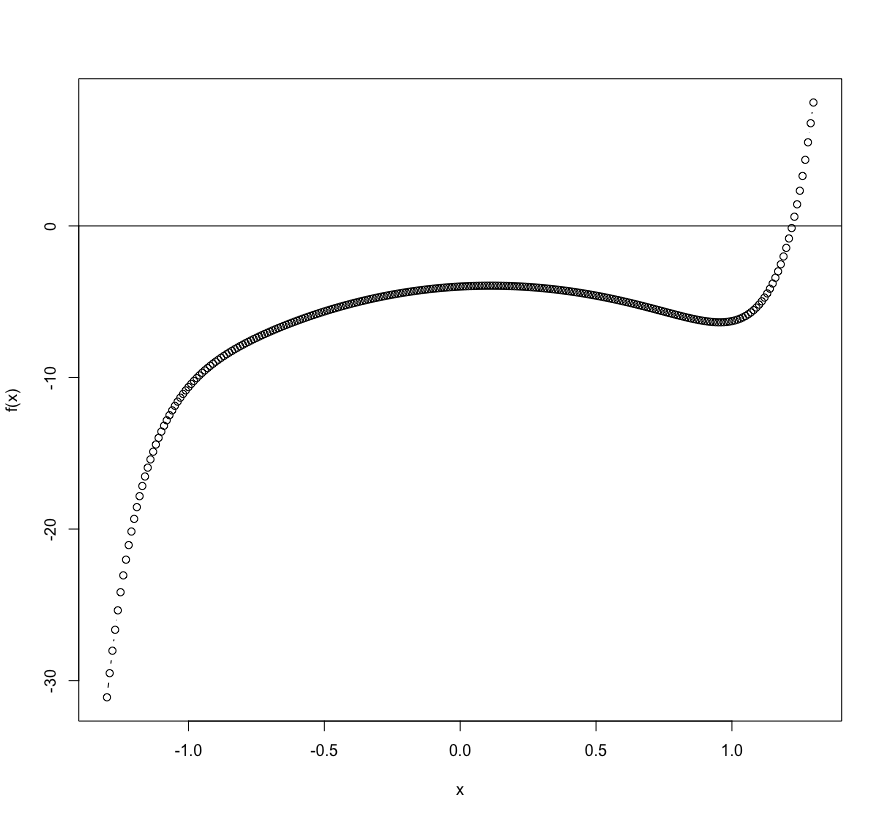
\includegraphics[width=1\textwidth]{plot1}
  \caption{Plot of function $f(x) = x^{11}-5x^2+e^x-5$ in the range from -2 to 2.}
\end{figure}

\section{Code Listings}
All calculations were done in R \cite{rlanguage}.
\subsection{nderiv}
\begin{lstlisting}
  nderiv = function (f, x, h) (f(x+h)-f(x))/h
\end{lstlisting}

\subsection{newton}
\begin{lstlisting}
  newton = function (f, x, n) {
    for(i in 1:n){
      x <- x-f(x)/nderiv(f,x,0.0001)
    }
    return(x)
  }
\end{lstlisting}



\section{Numeric Solution of $x^{11}-5x^2+e^x=5$}
From the graph in exercise 1, $x = -1$ was chosen as start value for the \verb+newton+ program.
The iteration was run with $n = \{1,10,100\}$ which resultet for the two latter values in an approximation of $y = -1.3667$.
\section{Local minima of $f(x) =^{11}-5x^2+e^x-5$}
\section{Find $f^{-1}(3)$ where $f(x) = x^{11}-5x^2+e^x-5$}
  
 
\addcontentsline{toc}{section}{\refname}
\bibliography{references}

\end{document}
